\documentclass[11pt]{article}
\usepackage{amsmath,amsthm,amssymb,fullpage,graphicx,hyperref,listings}
\usepackage{listings,color,setspace}
\author{Andy Reagan}
\title{Math 337 Homework 12}

     \def\NN{\mathbb{N} }
     \def\ZZ{\mathbb{Z} }
     \def\QQ{\mathbb{Q} }
     \def\RR{\mathbb{R} }
     \def\CC{\mathbb{C} }
     \def\f{\frac }
     \def\b{\begin }
     \def\e{\end }
     \def\Log{\text{Log} \,}
     \def\Re{\text{Re} \, }

\lstset{language=MATLAB,
basicstyle=\ttfamily\scriptsize\singlespacing,
keywordstyle=\color{black},
stringstyle=\color{black},
commentstyle=\color{black},
morecomment=[l][\color{black}]{\#},
frame=L,
xleftmargin=\parindent,
%%numbers=left,                   %% where to put the line-numbers
%%numberstyle=\scriptsize,      %% the size of the fonts that are used for the line-numbers
%%stepnumber=1,                   %% the step between two line-numbers. If it is 1 each line will be numbered
numbersep=5pt,
breaklines=true,        %% sets automatic line breaking
breakatwhitespace=false,    %% sets if automatic breaks should only happen at whitespace
escapeinside={\%*}{*)} 
}


     \newcommand{\pdiff}[2]{\frac{\partial #1}{\partial #2}}
     \newcommand{\partialdiff}[2]{\frac{\partial #1}{\partial #2}}
     \newcommand{\pdiffsq}[2]{\frac{\partial^2 #1}{{\partial #2}^2}}
     \newcommand{\pdiffcu}[2]{\frac{\partial^3 #1}{{\partial #2}^3}}
     \newcommand{\pdiffhi}[3]{\frac{\partial^#3 #1}{{\partial #2}^#3}}
     \newcommand{\diff}[2]{\frac{{\rm d}#1}{{\rm d}#2}}
     \newcommand{\diffsq}[2]{\frac{{\rm d}^{2}#1}{{\rm d} {#2}^2}}
     \newcommand{\diffhi}[3]{\frac{{\rm d}^#3 #1}{{\rm d} {#2}^#3}}
     \newcommand{\tdiff}[2]{\mbox{d} #1/\mbox{d} #2}
     \newcommand{\tdiffsq}[2]{\mbox{d}^{2} #1/\mbox{d} {#2}^2}
     \newcommand{\tpdiff}[2]{\partial #1/\partial #2}
     \newcommand{\tpdiffsq}[2]{\partial^2 #1/\partial {#2}^2}
     \newcommand{\bvec}[1]{\vec{ {\bf #1 } }}
     \newcommand{\oh}[1]{O(h^{{#1}})}

\begin{document}
\maketitle

\begin{enumerate}

\item I code up the scheme from (12.12) on the IBVP (12.1-12.3) in the notes.

We observe that the solution is accurate for $h = 0.1, \kappa = 0.004$, which agrees with the condition that $\kappa < 0.5 \cdot h^2$, from Eq (12.17). When $h$ is decreased, I expect that the solution may no longer be stable since the above condition is not satisfied.

Indeed this is what we find.

\lstinputlisting[language=Matlab]{andy_hw12_prb01.m}

\begin{figure}[h!]
  \centering
    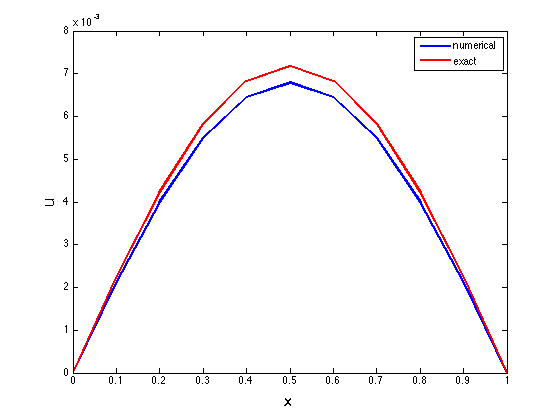
\includegraphics[width=0.45\textwidth]{andy_hw12_prb01_02.png}
  \caption{The numerical and exact solution for $h=0.1$.}
\end{figure}

\begin{figure}[h!]
  \centering
    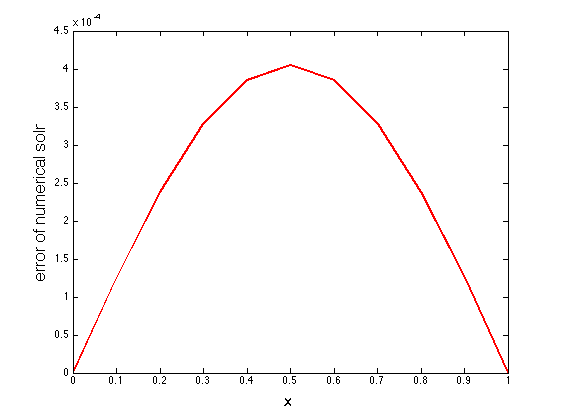
\includegraphics[width=0.45\textwidth]{andy_hw12_prb01_03.png}
  \caption{The error for $h=0.1$.}
\end{figure}

\begin{figure}[h!]
  \centering
    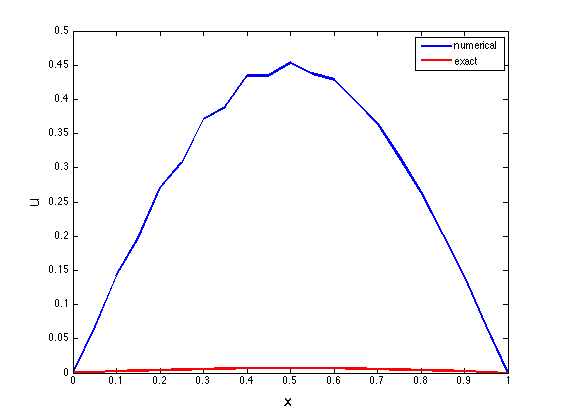
\includegraphics[width=0.45\textwidth]{andy_hw12_prb01_05.png}
  \caption{The numerical and exact solution for $h=0.05$.
           Since the stability condition on $\kappa$ (12.17) is no longer satisfied, the solution behaves badly.
           My code stops when the minimax principle is violated.}
\end{figure}

\begin{figure}[h!]
  \centering
    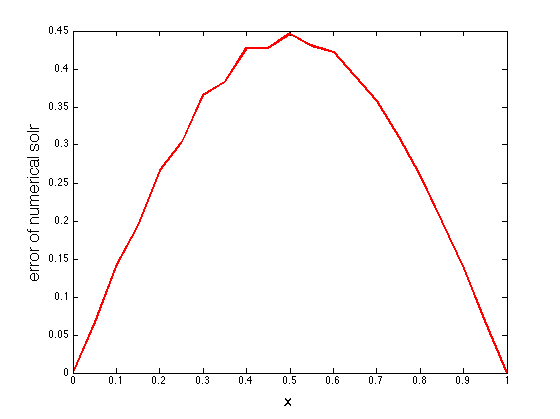
\includegraphics[width=0.45\textwidth]{andy_hw12_prb01_06.png}
  \caption{The error for $h=0.05$.}
\end{figure}

\clearpage
\pagebreak
\item From the notes we have that the Eigenvalues of a tridiagonal matrix are
\[ \lambda _j = b + 2\sqrt{ac} \cos \left ( \f{\pi j} {M} \right ) ,~~~~~~~~j = 1,\ldots,M-1.\]
From Eq. (12.15), this becomes
\[ \lambda _j = -\f{2}{h^2} + 2s\sqrt{\left( \f{1}{h^2}\right) \left ( \f{1}{h^2} \right )} \cos \left ( \f{\pi j} {M} \right ) =  -\f{2}{h^2} + \left ( \f{2}{h^2} \right ) \cos \left ( \f{\pi j} {M} \right ) ,~~~~~~~~j = 1,\ldots,M-1.\]
Since the method is Simple Euler, we require that these real Eigenvalues (since $A$ is symmetric, they are additionally gauranteed to be real) are bounded by $[-2,0]$ (when mutliplied by the stepsize, i.e. we need to bound $\lambda \kappa$).
Specifically, we require that $\lambda_{\min} > -2$ and $\lambda _{\max} < 0$.

Intuitvely obvious to the casual observer, the above $\lambda _j$ is maximum (closest to 0) when $\cos \left ( \f{\pi j} {M} \right ) $ is closest to $1$, which occurs at $j = 1$.
Since $\cos \left ( \f{\pi } {M} \right ) $ is less than 1, we observe that $\lambda _{\max} < 0$.

Now for $\lambda_{\min}$, we need to be more careful.
In particular, $\lambda _j$ is minimal when $\cos \left ( \f{\pi j} {M} \right ) $ is closest to $-1$.
This occurs for $j = M-1$, and we have 
\[ \cos \left ( \f{\pi (M-1)} {M} \right ) = \cos \left ( \pi - \f{\pi}{M} \right ) \simeq -1 + \left( \f{-\pi}{M} \right) ^2 < -1 .\]
In particular
\[ \lambda _{\min} \simeq \f{-2}{h^2} + \f{2}{h^2} \left ( -1 + \f{\pi^2}{M^2} \right ) = -\f{4}{h^2} + \f{\pi^2}{M^2} .\]
Therefore
\[ \kappa \lambda _{\min} > -\f{4\kappa}{h^2} = -4r .\]
Since $M$ is large, we note that while the above inequality always holds (necessarily), the difference is very small, so $\kappa \lambda _{\min} \simeq -4r$ itself.
Recalling that we require $\kappa \lambda _{\min} > -2$, we have $-4r > -2 \Rightarrow r< 1/2$.

\clearpage
\pagebreak
\item The difference scheme is (equating the approximations for $u_{xx}$ and $u_t$ per the Heat equation):
\[ U_{m} ^{n+1} = U_{m} ^{n-1} +2( r U_{m+1} ^{n} -2r U_{m} ^{n} + r U_{m-1} ^{n}) .\]

The stencil is:

\begin{figure}[h!]
  \centering
    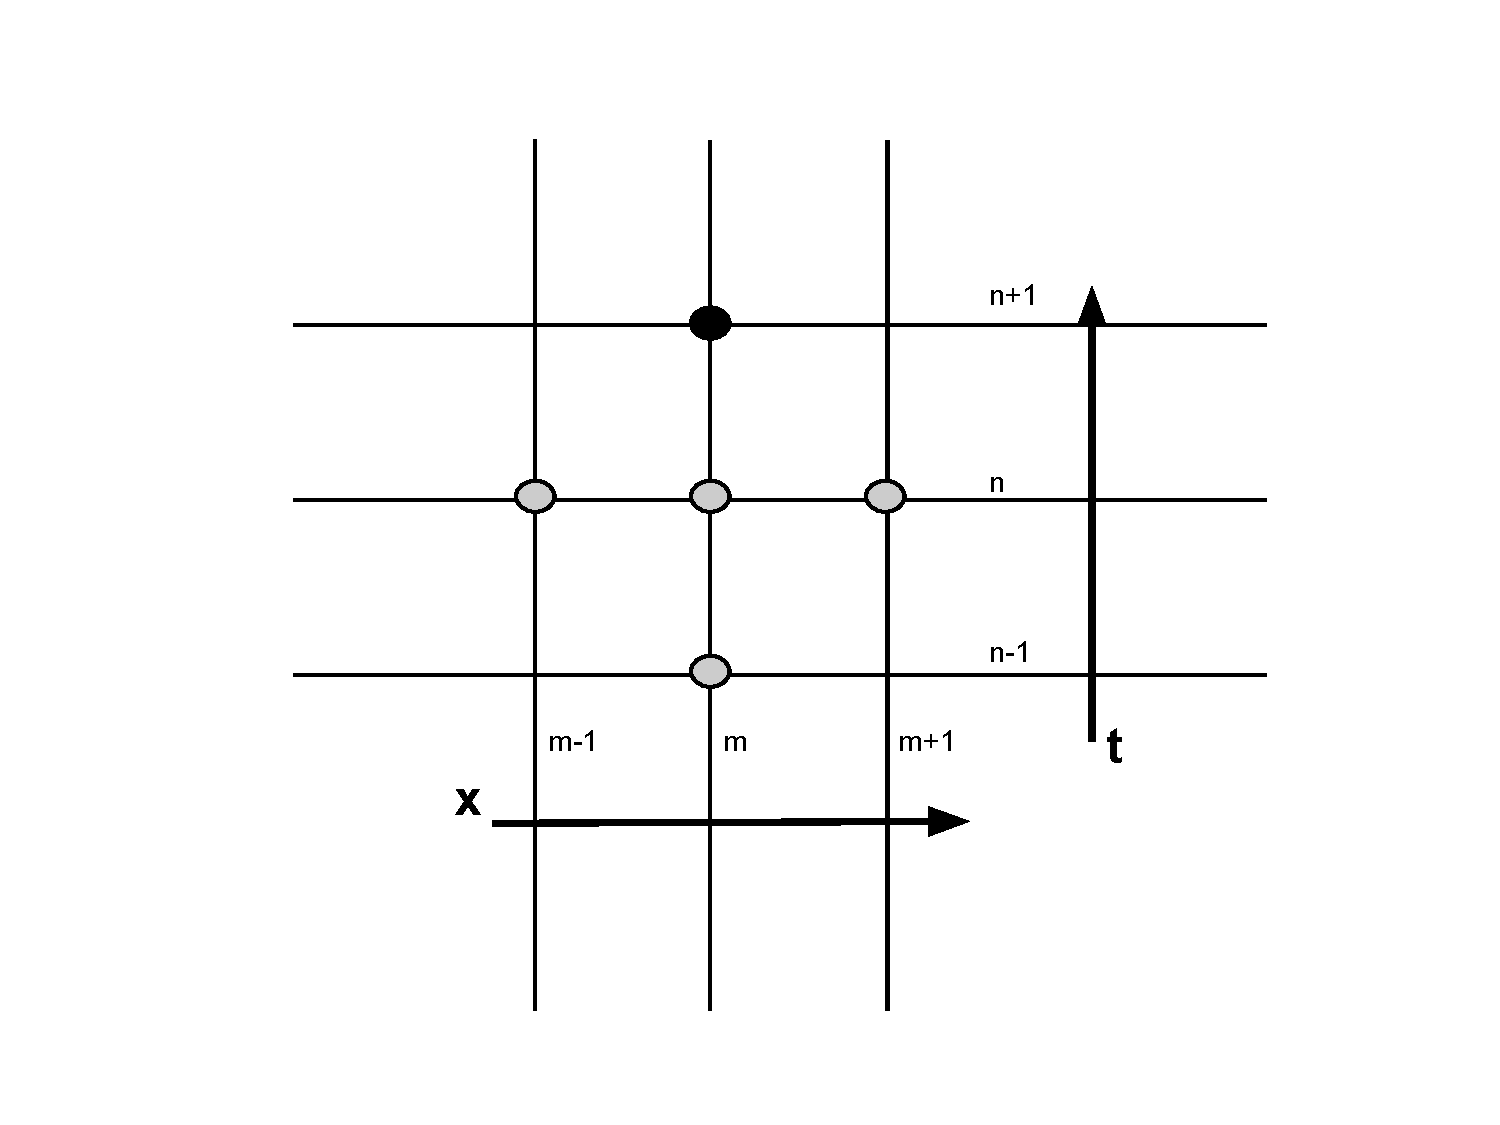
\includegraphics[width=0.45\textwidth]{337_hw12_03.pdf}
  \caption{The stencil for the ``Leap-Frog'' PDE scheme.}
\end{figure}

Applying the von Neumann stability analysis, we start with the error statisfying the (linear) difference scheme:
\[ \epsilon_{m} ^{n+1} = \epsilon_{m} ^{n-1} + 2 ( r \epsilon_{m+1} ^{n} -2r \epsilon_{m} ^{n} + r \epsilon_{m-1} ^{n} ).\]
We expand $\epsilon$ as a Fourier series, specifically
\[ \epsilon _n ^m = \sum _l c_l (n) e^{i\beta _l x_m} .\]
Since we are interested in studying the grow of this error, we look for $c_l$ of the form $\rho _l ^n$, to discover the exponential behavior.
Fixing $l$, we expand the error difference scheme in the chosen spectral basis as
\[ \rho ^{n+1} e^{i \beta m h} = \rho ^{n-1} e^{i \beta m h} + 2( \rho ^{n} e^{i \beta (m+1) h} -2 \rho ^{n} e^{i \beta m h} + \rho ^{n} e^{i \beta (m-1) h}) .\]
Cancelling $\rho ^{n} e^{i \beta m h}$, and redifining $r = 2\kappa / h^2,$ we are left
\[ \rho^2 = 1 + \rho \left ( r e^{i\beta h} -2r + re^{-i\beta h } \right ) = 1 + \rho z \]
where from the hint we have rewritten $z$ as
\[ z = -4r \sin ^2 \left ( \f{\beta h }{2} \right ) .\]
Given that we want to show this scheme is unstable for $z\ne 0$ we need to show that $|\rho | > 1$ for $z \ne 0$.
In particular, from the equation $\rho ^2 = 1 + \rho z$ we have that
\[ \rho = \f{z \pm \sqrt{z^2 + 4} }{2} \simeq \f{z \pm 2 \pm z/2 }{2} = \left \{ 3z/4 +  1 , z/4 - 1 \right \} .\]
For $\beta h$ taking on any value, it is possible that $z$ is positive or negative (or 0).
Regardless of the sign of $z$ (if it is nonzero), one of the above $\rho$ has magnitude greater than 0, hence this scheme is unstable.
In particular, for $z<0$ the root $\rho = -1 + z/4 < -1$ and for $z>0$ the root $\rho = 3z/4+1 > 1$.

However, for $z = 0$, $|p| = 1$ so we cannot deem this scheme to be explicity unstable for the model problem.

The scheme is an analog (in terms of method, and stability region) the Leap-Frog method for ODE's.

\item (a) Since the difference scheme is linear, the error obeys the same equation, and we plug $\epsilon _{m} ^{n}$ into the given scheme:

\begin{align} \overline{\epsilon} _m &= r \epsilon _{m} ^{n} + (1-2r) \epsilon _{m} ^{n} + r \epsilon _{m-1} ^{n}\\
\epsilon _{m} ^{n+1} &=  \epsilon _{m} ^{n} + \f{r}{2} \left [ \left ( \epsilon _{m+1} ^{n} -2 \epsilon _{m} ^{n} + \epsilon _{m-1} ^{n} \right ) + \left ( \overline{\epsilon} _{m+1} ^{n} -2 \overline{\epsilon} _{m} ^{n} + \overline{\epsilon} _{m-1} ^{n} \right ) \right ]\end{align}

Using the same Fourier expansion as Problem 3 (again expanding only one value of $l$ and assuming $c_l (n) = \rho_l ^n$, we have
\begin{align} \overline{\epsilon} _{m+1} &= r\rho ^{n} e^{i \beta (m+2) h}  + (1-2r) \rho ^{n} e^{i \beta (m+1) h} + r \rho ^{n} e^{i \beta m h}\\
&= \rho ^{n} e^{i \beta (m+1) h}  \left ( 1+  r \left (  e^{i \beta h} - 2 + e^{-i \beta h} \right ) \right ) \\ 
&= \rho ^{n} e^{i \beta (m+1) h}  \left ( 1+  z \right ) \\ 
\overline{\epsilon} _{m} &= \rho ^{n} e^{i \beta m h}  \left ( 1+  z \right ) \\ 
\overline{\epsilon} _{m-1} &= \rho ^{n} e^{i \beta (m-1) h}  \left ( 1+  z \right ) \end{align}

We now have the
\begin{align*} \rho ^{n+1} e^{i \beta (m) h} &= \rho ^{n} e^{i \beta (m) h} + \f{r}{2} \left ( \rho ^{n} e^{i \beta (m+1) h} -2 \rho ^{n} e^{i \beta (m) h} + \rho ^{n} e^{i \beta (m-1) h} + (1+z) \rho ^{n} e^{i \beta (m+1) h} \right.\\
&~~~~~ \left. -2 (1+z) \rho ^{n} e^{i \beta (m) h} + (1+z) \rho ^{n} e^{i \beta (m-1) h} \right ) \\
&= \rho ^{n} e^{i \beta (m) h} + \f{r}{2} \left ( (2+z) \rho ^{n} e^{i \beta (m+1) h} -2 (2+z) \rho ^{n} e^{i \beta (m) h} + (2+z) \rho ^{n} e^{i \beta (m-1) h} \right ) \\
&= \rho ^{n} e^{i \beta (m) h} + \f{r}{2} (2+z) \rho ^{n} e^{i \beta m h}\left (  e^{i \beta h} -2 + e^{-i \beta h} \right ) \\
&= \rho ^{n} e^{i \beta (m) h} + \f{r}{2} (2+z) \rho ^{n} e^{i \beta m h}\left (  \f{z}{r} \right ) \\
&= \rho ^{n} e^{i \beta (m) h} + \f{z}{2} (2+z) \rho ^{n} e^{i \beta m h}\end{align*}

Cancelling the $e^{i \beta m h}$, and we have
\begin{align*} \rho ^{n+1} &= \rho ^n + \rho ^n \left (\f{z^2}{2} + z \right )\\
&= \rho^n \left (\f{z^2}{2} + z + 1\right )\end{align*}
And losing $\rho ^n$, we have
\begin{align*} \rho &= \f{z^2}{2} + z + 1\end{align*}
which indeed agrees with Eq 4.21.
We next bound $|\rho|$ less than 1, and since $f(z) = z^2/2 + z + 1 > 0$ for any $z$, we only need that $\rho < 1$.
Setting $f(z) = 1$, we clearly will have the roots 0 and -2, so our requirement that $|\rho| < 1 \Rightarrow -2<z<0$.

This requirement is:
\[ -2 < -4 r \sin ^2 \left (\f{\beta h}{2} \right ) < 0.\]

Since $\sin ^2 \in [0,1]$, and $r$ is positive, for $\sin ^2 \ne 0$ the RHS bound is satisfied.
We will revisit $\sin ^2 = 0$.

The left hand bound becomes
\begin{align*} -2 &< -4 r \sin ^2 \left (\f{\beta h}{2} \right )\\
\f{1}{2} &>  r \sin ^2 \left (\f{\beta h}{2} \right )\end{align*}
Again since $\sin ^2 \in [0,1]$, the most dangerous value of $\beta h$ is that which makes $\sin ^2 (\beta h /2) = 1$.
Specifically, this is $\beta = \pi / h$, corresponding the to the highest frequency mode on a grid of spacing $h$.
For this $\beta$, the above equation makes clear that $r < 1/2$ for stability.

(b) When $r > 1/2$, we will have $z < -2$, which makes $\rho > 1$.
Therefore, the error will grow as $\rho ^n$ at timestep $n$ with $\rho > 1$ (and increase monotonically).
For method 12.12, Eq 12.35 indicates that for $r > 1/2$ the ``$z$'' will again become less that $-2$.
However, since $\rho \simeq 1+z$, we will have $\rho < -1$.
Therefore, the error will grow as $\rho ^n = (-1)^n |\rho | ^n$ at timestep $n$ with $|\rho | > 1$ (and thus oscillate).

(c) Since $r = \kappa / h^2$, this is not the method you want.
Let's look at an example.
Fix $h = 0.1$, such that $h^2 = 0.01$, we require for stability that $\kappa / .01 < 1/2 \Rightarrow k < 0.005$.
Now $\kappa ^2 << h^2$ so $0(\kappa ^2 + h^2 ) \simeq O(h^2)$.

(d) I do not find the expected instability for $\kappa = 0.006$ here (like that of Problem 1), contradicting the above analysis.
My code is below.

\lstinputlisting[language=Matlab]{andy_hw12_prb04.m}

\item (a) I don't get this exact form, from what you've suggested.
Taking the $\log _{2}$ of both sides of Equation (2), we get
\[ \log _2 \left (\epsilon (x,h) \right ) = \gamma(x) \log_2 \left (Ch \right ) ,\]
where I have made explicit that $\epsilon$ depends on $h$.
If we consider only one value of $x$, we have
\[ \log _2 \left (\epsilon (x_m,h) \right ) = \gamma(x_m) \log_2 \left (Ch \right ) ,\]
and since our indepedent variable here is $h$, we notice the slope of $\log _2 (\epsilon (x_m , h) )$ over the axis of $\log _2 (Ch)$ has slope $1/\gamma(x_m)$.
Therefore, we can solve for $\gamma$ using the formula $(f(b)-f(a))/(b-a)$ where the points $a,b$ are $h,h/2$ inside of $\log _2 (Ch)$ and $f(h) = \log _2 (\epsilon (x_m , h) )$.
Putting this together, we have
\[ \gamma \simeq \f{\log _2 (Ch) - \log_2(Ch/2)}{\log_2 (\epsilon (h)) - \log_2 (\epsilon (h/2))} .\]

(b) I present the results in the following table:

\begin{table}[h]
  \begin{center}
    \begin{tabular}{cccc}
      \hline
      $p$ & $r = 0.5$ & $r=0.4$ & $r=0.3$ \\
      \hline
      \hline
      0  & N/A & 0.6676 & 0.9149 \\
      1  & N/A & 1.9932 & 2.0012 \\
      2  & 2.0653 & 1.9932 & 1.9872\\
      \hline
    \end{tabular}
  \end{center}
\end{table}

Conclusions from the table: (i) the accuracy increases dramatically as the smoothness increases (particularly for having at least 1 continuous derivative) and (ii) accuracy increases as $r$ decreases for less smooth IC, where for smooth IC it actually decreases, albeit very slightly.
In particular, for $r$ very close to the stability threshold the solution is unreliable for nonsmooth IC.

(c) For $p = 0, r = 0.5$, each value of $h$ is noticably jagged.
For $p = 1, r = 0.5$ only the value of $h = 0.05$ is jagged.
The jaggedness that we see is the most unstable mode, which shows up for this $r$ since it is close to the stability treshold, and the most unstable mode dominates the error.

(d) If the initial condition is non-smooth, and $h$ is fixed, it is necessary to choose $\kappa$ such that $r$ is not close to the stability threshold of $1/2$.
Choosing $\kappa$ such that $r = 0.4$ is appropriate for IC with at least one continuous derivative, but if even this is not known, then it is necessary to choose an even smaller $\kappa$, perhaps to make $r = 0.1$, so that the error scales close to linearly with the stepsize (for $r = 0.1$, we obtain that $\gamma \simeq 1.03$, for superlinear error decay with $h$, at $p = 0$).

\end{enumerate}

\end{document}



